\documentclass{article}
\usepackage[utf8]{inputenc}

\title{Opis naprawy robota mobilnego "RYŚ"}
\author{Kamil Foryszewski}

\usepackage{graphicx}

\begin{document}

\maketitle

\section{Diagnoza usterki}
W robocie mobilnym "RYŚ" doszło do uszkodzenia sterownika jednego z dwóch silników napędowych. Diagnoza rozpoczęła się od sprawdzenia odczytów z czujników znajdujących się w uszkodzonym sterowniku. Na tym etapie ustalono iż układ MAX485 odpowiedzialny za komunikację pomiędzy sterownikiem a komputerem nie działa prawidłowo. Kolejnym etapem było sprawdzenie działania analogowej części mocy sterownika składającej się z dwóch par tranzystorów MOSFET, oddzielonych od części logicznej za pomocą transoptorów. Po zmierzeniu napięć na bramkach tranzystorów oraz na wyjściach sterujących mikrokontrolera okazało się że transoptory nie działają prawidłowo. 

\section{Podjęte działania}
Ze względu na problematyczność wymiany uszkodzonych elementów, na bazie zapasowej płytki PCB, zmontowano nowy sterownik. Zostały w nim wprowadzone modyfikacje usprawniające pracę z robotem i poprawiające estetykę, jak np. złącza zasilające innego typu. Ponieważ do poprawnego działania robot potrzebuje dwóch identycznych mostków, to w drugim mostku zostały wymienione tranzystory MOSFET oraz wprowadzone zmiany analogicznie do poprzedniego.Dodatkowo zostały wymienione silniki napędowe, ponieważ podczas testów uzwojenie jednego z silników zostało częściowo uszkodzone. W rezultacie robot posiada dwa zespoły napędowe o identycznej charakterystyce pracy. Poniżej przedstawiono grafiki obrazujące dokonane zmiany. 

\begin{figure}[h!]
\centering
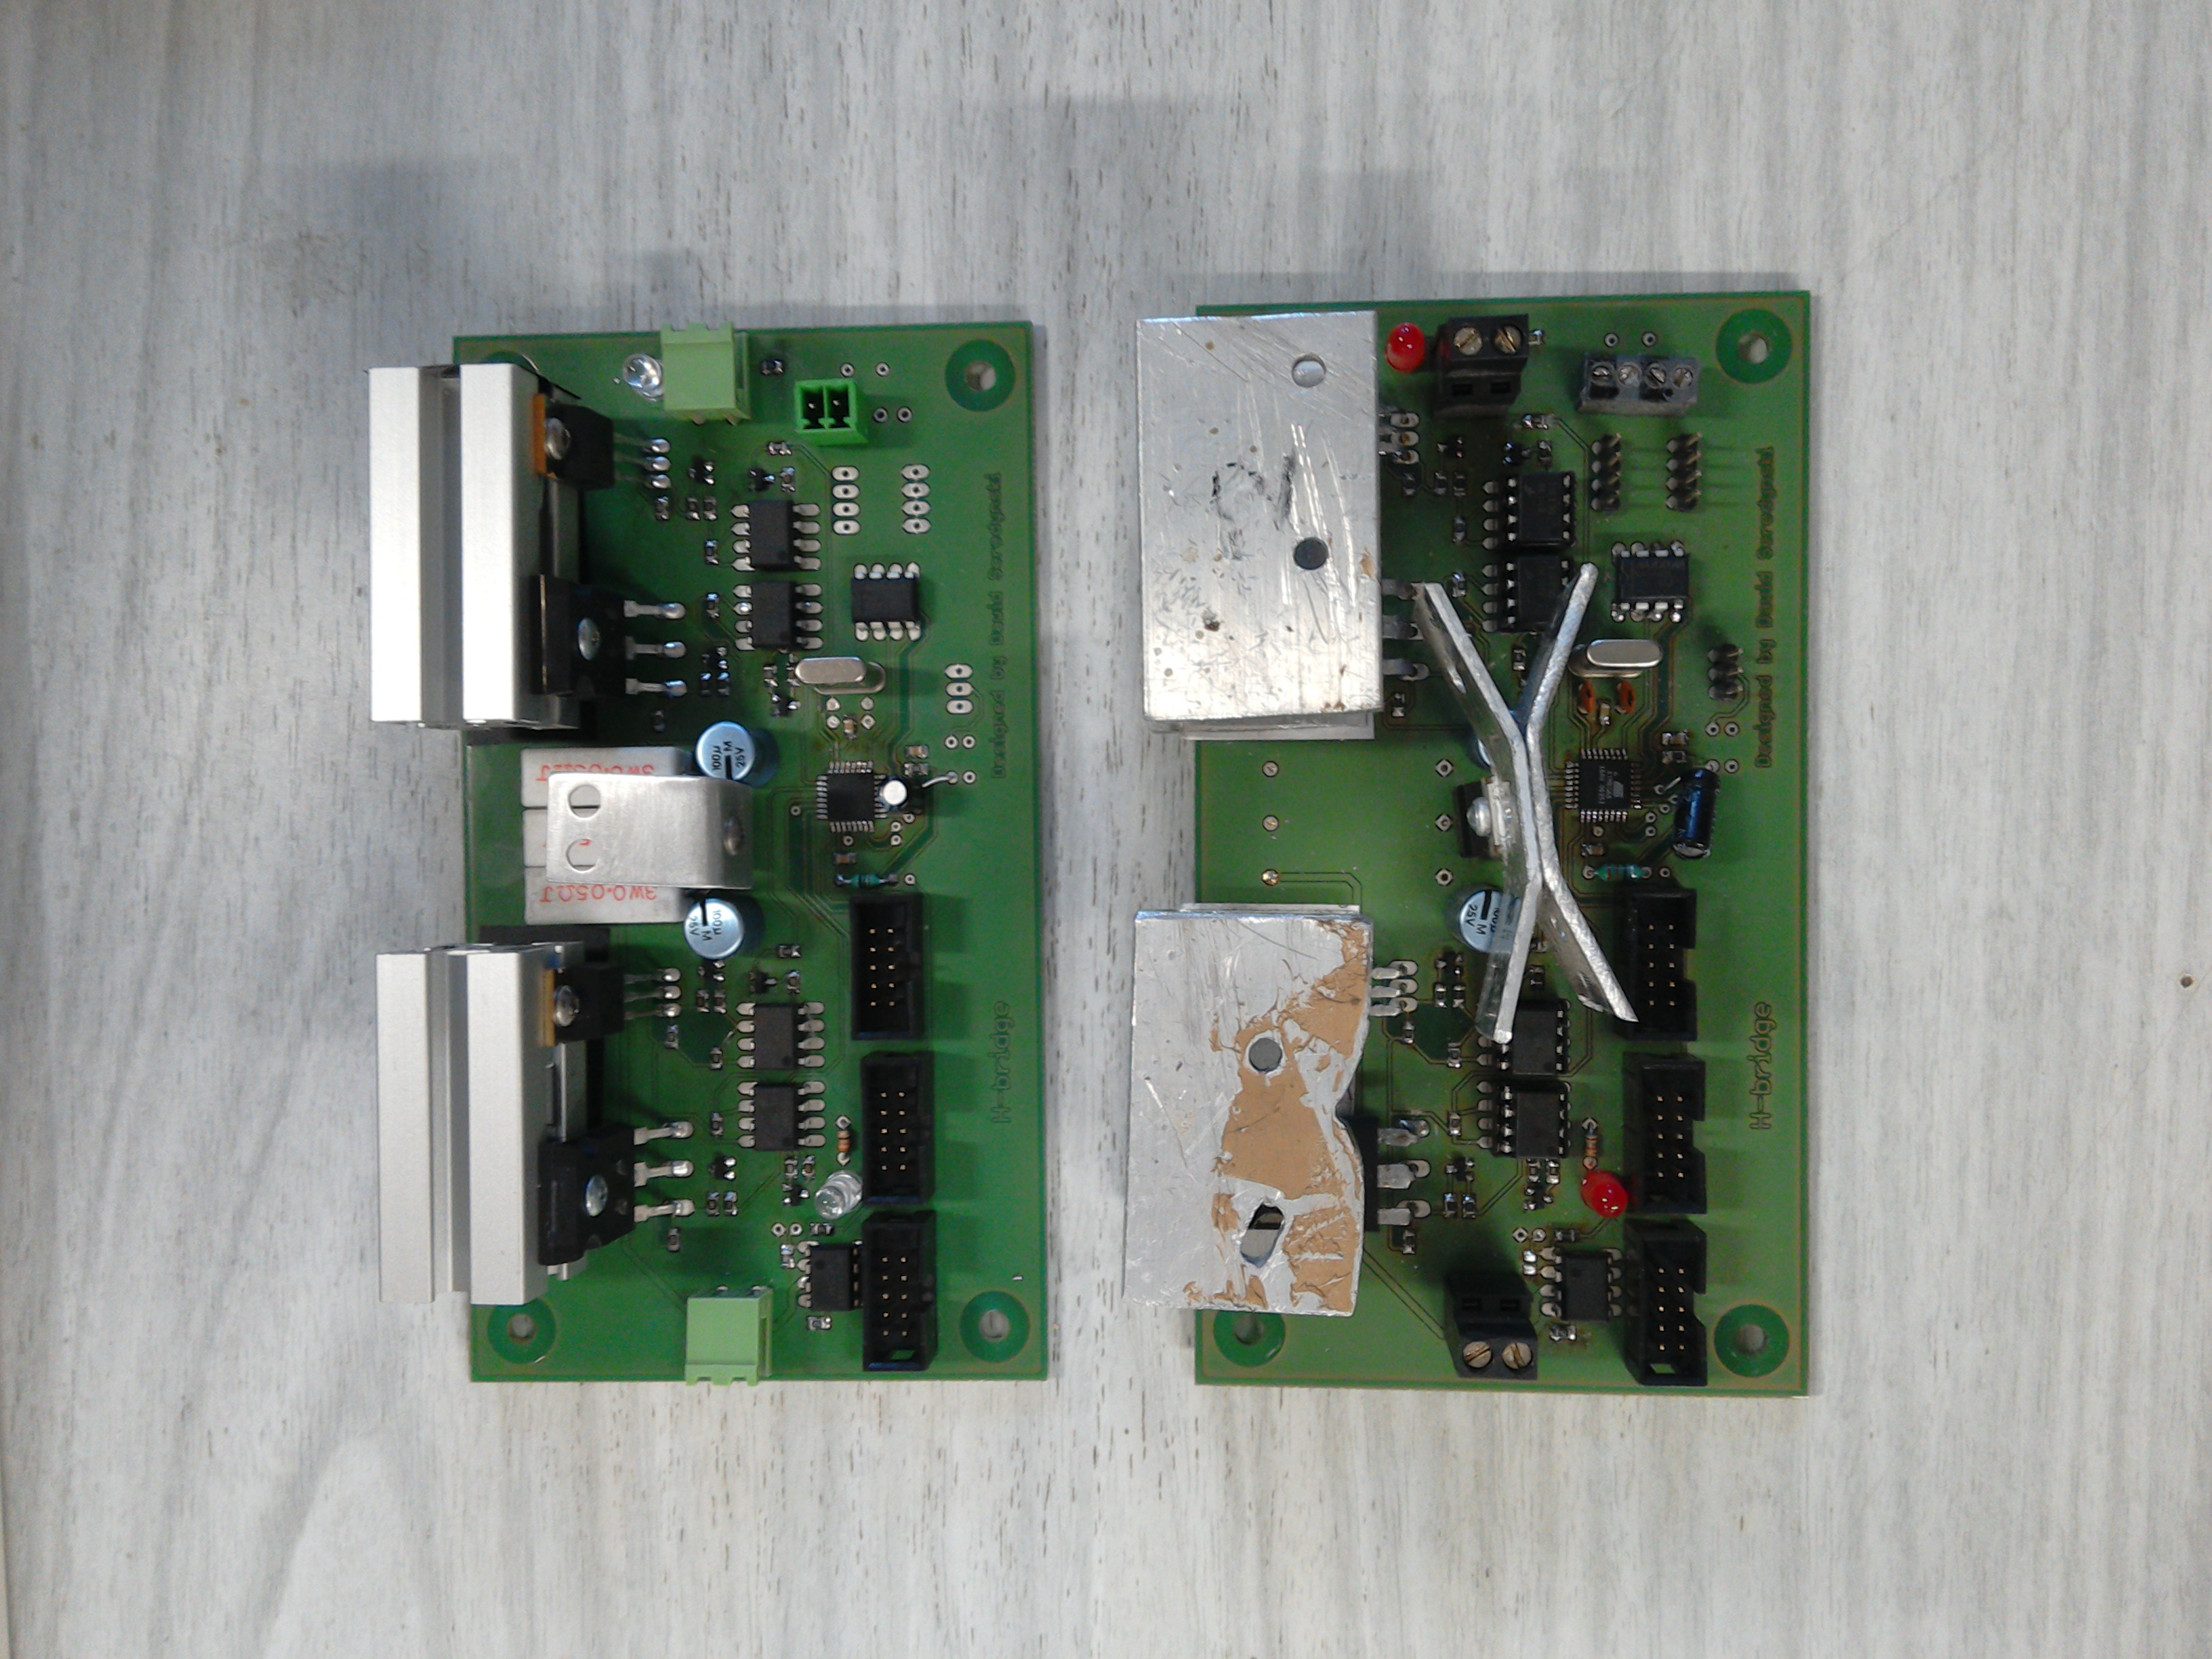
\includegraphics[scale=0.15 , angle=270, origin=c]{Drivers.jpg}
\caption{Sterownik nowy i stary}
\end{figure}

\begin{figure}[h!]
\centering
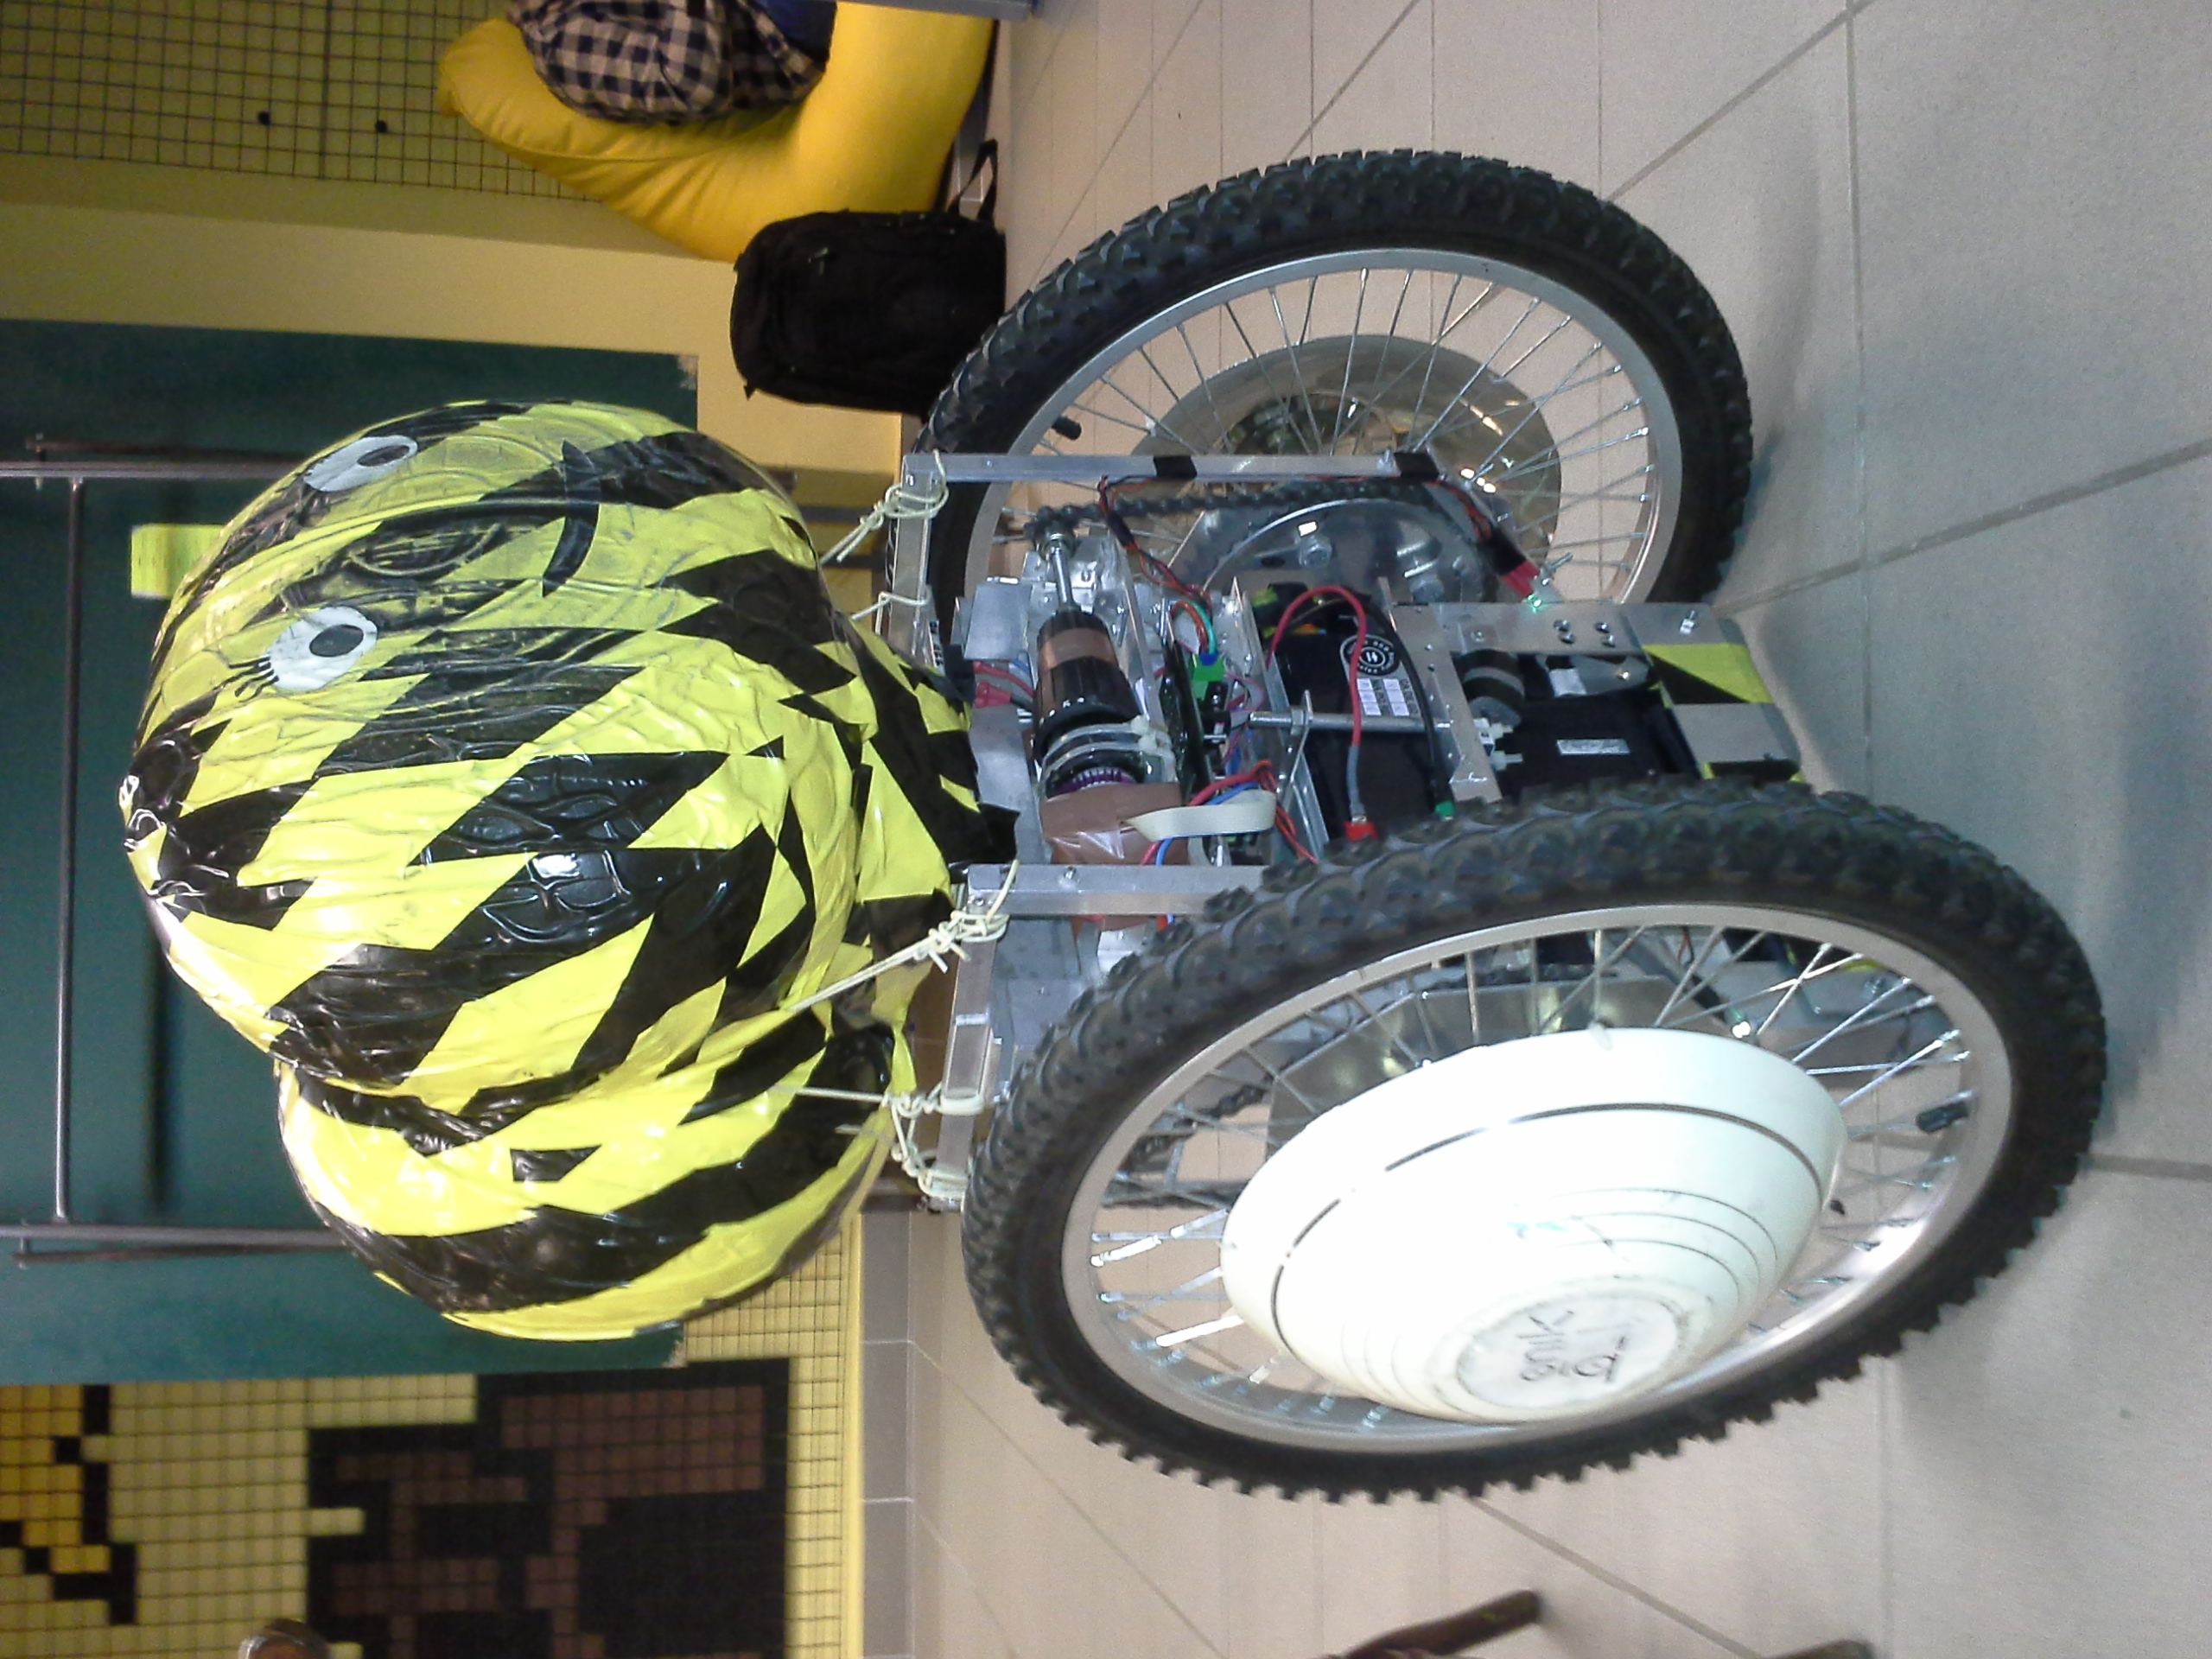
\includegraphics[scale=0.18 , angle=270, origin=c]{Robot.jpg}
\caption{Robot w stanie pracy}
\end{figure}

\end{document}
